% !TEX TS-program = xelatex
% !BIB program = bibtex
% !TeX spellcheck = ru_RU

% About magic macros see also
% https://tex.stackexchange.com/questions/78101/

% По умолчанию используется шрифт 14 размера.
% Если Вы не влезаете в лимит страниц и нужен 12-й шрифт,
% то уберите опцию [14pt]
\documentclass[14pt, russian]{matmex-diploma-custom}

% !TeX spellcheck = ru_RU
% !TEX root = vkr.tex
% Опциональные добавления используемых пакетов. Вполне может быть, что они вам не понадобятся, но в шаблоне приведены примеры их использования.
\usepackage{tikz} % Мощный пакет для создание рисунков, однако может очень сильно замедлять компиляцию
\usetikzlibrary{decorations.pathreplacing,calc,shapes,positioning,tikzmark}

% Библиотека для TikZ, которая генерирует отдельные файлы для каждого рисунка
% Позволяет ускорить компиляцию, однако имеет свои ограничения
% Например, ломает пример выделения кода в листинге из шаблона
% \usetikzlibrary{external}
% \tikzexternalize[prefix=figures/]

\newcounter{tmkcount}

\tikzset{
	use tikzmark/.style={
			remember picture,
			overlay,
			execute at end picture={
					\stepcounter{tmkcount}
				},
		},
	tikzmark suffix={-\thetmkcount}
}

\usepackage{booktabs} % Пакет для верстки "более книжных" таблиц, вполне годится для оформления результатов
% В шаблоне есть команда \multirowcell, которой нужен этот пакет.
\usepackage{multirow}
\usepackage{siunitx} % для таблиц с единицами измерений

\newcommand{\cd}[1]{\texttt{#1}}
\newcommand{\inbr}[1]{\left<#1\right>}

% Для названий стоит использовать \textsc{}
\newcommand{\OCaml}{\textsc{OCaml}}
\newcommand{\miniKanren}{\textsc{miniKanren}}
\newcommand{\BibTeX}{\textsc{BibTeX}}
\newcommand{\vsharp}{\textsc{V$\sharp$}}
\newcommand{\fsharp}{\textsc{F$\sharp$}}
\newcommand{\csharp}{\textsc{C$\sharp$}}
\newcommand{\GitHub}{\textsc{GitHub}}
\newcommand{\SMT}{\textsc{SMT}}

\newcolumntype{L}[1]{>{\raggedright\let\newline\\\arraybackslash\hspace{0pt}}m{#1}}
%\newcolumntype{C}[1]{>{\centering\let\newline\\\arraybackslash\hspace{0pt}}m{#1}}
\newcolumntype{R}[1]{>{\raggedleft\let\newline\\\arraybackslash\hspace{0pt}}m{#1}}

%  Команды и пакеты, не используемые в шаблоне, которые тем не менее могут быть полезными.

% \newcolumntype{Y}{>{\centering\arraybackslash}X}

% \usepackage{mathrsfs}

% \lstdefinelanguage{ocaml}{
% keywords={@type, function, fun, let, in, match, with, when, class, type,
% nonrec, object, method, of, rec, repeat, until, while, not, do, done, as, val, inherit, and,
% new, module, sig, deriving, datatype, struct, if, then, else, open, private, virtual, include, success, failure,
% lazy, assert, true, false, end},
% sensitive=true,
% commentstyle=\small\itshape\ttfamily,
% keywordstyle=\ttfamily\bfseries, %\underbar,
% identifierstyle=\ttfamily,
% basewidth={0.5em,0.5em},
% columns=fixed,
% fontadjust=true,
% literate={->}{{$\to$}}3 {===}{{$\equiv$}}1 {=/=}{{$\not\equiv$}}1 {|>}{{$\triangleright$}}3 {\\/}{{$\vee$}}2 {/\\}{{$\wedge$}}2 {>=}{{$\ge$}}1 {<=}{{$\le$}} 1,
% morecomment=[s]{(*}{*)}
% }

\usepackage{totcount}
\usepackage{setspace}
\usepackage{indentfirst}
\usepackage{hyperref}


\begin{document}
% TODO: Formatting
% % !TeX spellcheck = ru_RU
% !TEX root = vkr.tex

%% Если что-то забыли, при компиляции будут ошибки Undefined control sequence \my@title@<что забыли>@ru
%% Если англоязычная титульная страница не нужна, то ее можно просто удалить.
\filltitle{ru}{
    %% Актуально только для курсовых/практик. ВКР защищаются не на кафедре а в ГЭК по направлению,
    %%   и к моменту защиты вы будете уже не в группе.
    chair              = {Кафедра системного программирования},
    group              = {21.Б07-мм},
    %
    %% Макрос filltitle ненавидит пустые строки, поэтому обязателен хотя бы символ комментария на строке
    %% Актуально всем.
    title              = {Динамическая бинарная трансляция в RISC-V c помощью instrew},
    %
    %% Здесь указывается тип работы. Возможные значения:
    %%   production - производственная практика;
    %%   coursework - отчёт по курсовой работе (ОБРАТИТЕ ВНИМАНИЕ, у техпрога и ПИ нет курсовых, только практики);
    %%   practice - отчёт по учебной практике;
    %%   prediploma - отчёт по преддипломной практике;
    %%   master - ВКР магистра;
    %%   bachelor - ВКР бакалавра.
    type               = {practice},
    %
    %% Здесь указывается вид работы. От вида работы зависят критерии оценивания.
    %%   solution - «Решение». Обучающемуся поручили найти способ решения проблемы в области разработки программного обеспечения или теоретической информатики с учётом набора ограничений.
    %%   experiment - «Эксперимент». Обучающемуся поручили изучить возможности, достоинства и недостатки новой технологии, платформы, языка и т. д. на примере какой-то задачи.
    %%   production - «Производственное задание». Автору поручили реализовать потенциально полезное программное обеспечение.
    %%   comparison - «Сравнение». Обучающемуся поручили сравнить несколько существующих продуктов и/или подходов.
    %%   theoretical - «Теоретическое исследование». Автору поручили доказать какое-то утверждение, исследовать свойства алгоритма и т.п., при этом не требуя написания кода.
    kind               = {solution},
    %
    author             = {Михайлов Илья Игоревич},
    %
    %% Актуально только для ВКР. Указывается код и название направления подготовки. Типичные примеры:
    %%   02.03.03 \enquote{Математическое обеспечение и администрирование информационных систем}
    %%   02.04.03 \enquote{Математическое обеспечение и администрирование информационных систем}
    %%   09.03.04 \enquote{Программная инженерия}
    %%   09.04.04 \enquote{Программная инженерия}
    %% Те, что с 03 в середине --- бакалавриат, с 04 --- магистратура.
    specialty          = {02.03.03 \enquote{Математическое обеспечение и администрирование информационных систем}},
    %
    %% Актуально только для ВКР. Указывается шифр и название образовательной программы. Типичные примеры:
    %%   СВ.5162.2020 \enquote{Технологии программирования}
    %%   СВ.5080.2020 \enquote{Программная инженерия}
    %%   ВМ.5665.2022 \enquote{Математическое обеспечение и администрирование информационных систем}
    %%   ВМ.5666.2022 \enquote{Программная инженерия}
    %% Шифр и название программы можно посмотреть в учебном плане, по которому вы учитесь.
    %% СВ.* --- бакалавриат, ВМ.* --- магистратура. В конце --- год поступления (не обязательно ваш, если вы были в академе/вылетали).
    programme          = {СВ.5162.2020 \enquote{Технологии программирования}},
    %
    %% Актуально всем.
    %% Должно умещаться в одну строчку, допускается использование сокращений, но без переусердствования,
    %% короткая строка с большим количеством сокращений выглядит странно
    %supervisorPosition = {проф. кафeдры системного программирования, д.ф.-м.н.,}, % Терехов А. Н.
    %supervisorPosition = {ст. преподаватель кафедры ИАС, к.~ф.-м.~н. (если есть),}, % Смирнов К. К.
    supervisorPosition = {ассистент кафедры системного программирования,},
    supervisor         = {Косарев~Д.~С.},
    %
    %% Актуально только для практик и курсовых. Если консультанта нет или он совпадает с научником, закомментировать или удалить вовсе.
    % consultantPosition = {должность, ООО \enquote{Место работы}, степень  (если есть),},
    % consultant         = {Консультант~К.~К.},
    %
    %% Актуально только для ВКР.
    % reviewerPosition   = {должность, ООО \enquote{Место работы}, степень (если есть),},
    % reviewer           = {Рецензент~Р.~Р.},
}

% Английский титульник нужен только для ВКР, остальные виды работ могут его смело игнорировать.
% \filltitle{en}{
%     chair              = {Advisor's chair},
%     group              = {ХХ.BХХ-mm},
%     title              = {Template for SPbU qualification works},
%     type               = {bachelor},
%     author             = {FirstName Surname},
%     %
%     %% Possible choices:
%     %%   02.03.03 \foreignquote{english}{Software and Administration of Information Systems}
%     %%   02.04.03 \foreignquote{english}{Software and Administration of Information Systems}
%     %%   09.03.04 \foreignquote{english}{Software Engineering}
%     %%   09.04.04 \foreignquote{english}{Software Engineering}
%     %% Те, что с 03 в середине --- бакалавриат, с 04 --- магистратура.
%     specialty          = {02.03.03 \foreignquote{english}{Software and Administration of Information Systems}},
%     %
%     %% Possible choices:
%     %%   СВ.5162.2020 \foreignquote{english}{Programming Technologies}
%     %%   СВ.5080.2020 \foreignquote{english}{Software Engineering}
%     %%   ВМ.5665.2022 \foreignquote{english}{Software and Administration of Information Systems}
%     %%   ВМ.5666.2022 \foreignquote{english}{Software Engineering}
%     programme          = {СВ.5162.2020 \foreignquote{english}{Programming Technologies}},
%     %
%     %% Note that common title translations are:
%     %%   кандидат наук --- C.Sc. (NOT Ph.D.)
%     %%   доктор ... наук --- Sc.D.
%     %%   доцент --- docent (NOT assistant/associate prof.)
%     %%   профессор --- prof.
%     supervisorPosition = {Sc.D, prof.},
%     supervisor         = {S.S. Supervisor},
%     %
%     consultantPosition = {position at \foreignquote{english}{Company}, degree if present},
%     consultant         = {C.C. Consultant},
%     %
%     reviewerPosition   = {position at \foreignquote{english}{Company}, degree if present},
%     reviewer           = {R.R. Reviewer}, }

% \maketitle
\setcounter{tocdepth}{2}
% \tableofcontents

% % !TeX spellcheck = ru_RU
% !TEX root = vkr.tex

\section*{Введение}
\thispagestyle{withCompileDate}

\paragraph{} Системы сборки --- это неотъемлемая часть разработки программного обеспечения, так как позволяет автоматизировать некоторые однотипные задачи, освобождая ресурсы на что-то другое. Системы сборки также применяются для создания конкретных образов конфигурируемых ОС, которые включают необходимые для какой-либо задачи модули. Представителем такого класса ОС является ОСРВ (операционная система реального времени) Embox, которая использует систему сборки Mybuild.

% Системы сборки являются довольно сложным программным продуктом. Mybuild написана на языке Makefile и состоит из следующих  библиотек функций - расширения языка Makefile
% Можно привести несколько примеров систем сборок: Makefile, CMake, Ninja, Dune, Meson. Основная задача системы сборки - это
Можно сформулировать задачу системы сборки так: собрать актуальную версию проекта на основе зависимостей между его частями и данных об их изменении, выполнив минимум задач по перекомпилированию \cite{mokhov2018build}. Главный пример системы сборки - это GNU Make, написанный на языке C и повсеместно использующийся на Unix-подобных ОС. Результатом работы некоторых систем сборки являются make-файлы, что позволяет повысить уровень абстракции при описании зависимостей. Примером таких систем являются CMake, Meson и Mybuild.

Реализация Mybuild написана на языке GNU Make, из-за чего возникают проблемы с масштабированием данной системы. Также код плохо задокументирован, в следствие чего работать с данным проектом становится затруднительно.

Предлагается провести реинжиниринг системы сборки Mybuild, а именно написать реализацию на функциональном языке OCaml.
% Формат из 4х частей рекомендуется в курсе Д.~Кознова~\cite{koznov} по написанию текстов.
% Части (абзацы) должны занять максимум на две страницы.
% \begin{enumerate}
% 	\item Известная информация (background/обзор).
% 	\item Неизвестная информация (пробел в знаниях).
% 	\item Гипотезы, вопросы, цели.
% 	\item Подход, план решения задачи, предлагаемое решение.
% \end{enumerate}

% Последний абзац должен читаться и быть понятен в отрыве от других трёх. Никакие абзацы нумеровать нельзя.

% С.-П. Джонс~\cite{SPJGreatPaper} предлагает несколько другой формат написания введения.
% Вполне возможно, что если Ваша работа про языки программирования, то его формат будет удачнее.

% \blfootnote{
% 	Иногда рецензенту полезно знать какого числа компилировался текст, чтобы оценить актуальность версии текста. В этом случае полезно вставлять в текст дату сборки. Для совсем официальных релизов документа это не вполне канон.\\
% 	Также здесь имеет смысл указать, если работа сделана на деньги, например, Российского Фонда Фундаментальных Исследований (РФФИ) по гранту номер такой-то, и т.п.}

% Embox - это кофигурируемая операционная система реального времени, которая применяется для embedded-систем.
% Mybuild - это система сборки для конфигурируемой операционной системы Embox, реализация которой написана на Makefile.
% Она состоит из двух декларативных языков программирования: Configfile, который отвечает за описание модулей, которые необходимо включить в сборку операционной системы, и Myfile, который ...
% Зачем нужна своя система сборки, когда есть CMake например???

% !TeX spellcheck = ru_RU
% !TEX root = vkr.tex

\section{Постановка задачи}
\label{sec:task}
Целью работы является реинжиниринг системы сборки Mybuild. Для её выполнения были поставлены следующие задачи:
\begin{itemize}
	\item осенний семестр: \begin{enumerate}
		      \item реализовать парсер декларативного языка Myfile;
		      \item протестировать парсер языка Myfile на существующей кодовой базе;
	      \end{enumerate}
	\item весенний семестр: \begin{enumerate}
		      \item реализовать парсер декларативного языка Configfile;
		      \item реализовать генерацию makefile'ов и других небходимых компонентов для сборки Embox;
		      \item провести тестирование.
	      \end{enumerate}
\end{itemize}
% Дословно \enquote{Целью работы является... Для её выполнения были постав\-лены следующие задачи:}
% \begin{enumerate}
% 	\item  реализовать это (раздел~\ref{subsec:task1});
% 	\item  спроектировать то-то (раздел~\ref{subsec:task2}) наилучшим образом;
% 	\item  протестировать на том-то (раздел~\ref{subsec:task3}) и обогнать тех-то;
% 	\item \sout{изучить язык \OCaml{}} писать тут не надо, так как тут должны быть задачи, выполнение которых можно проверить/оценить прочитав текст или выслушав доклад;
% 	      (т.е. Ваши достижения должны быть опровержимы)
% 	      \begin{itemize}
% 		      \item \sout{произведен обзор предметной области} не нужно писать по той же причине. \emph{Исключение: вы опубликовали обзорную статью и готовы её предъявить как доказательство проведенного обзора.}
% 	      \end{itemize}
% \end{enumerate}

% % !TeX spellcheck = ru_RU
% !TEX root = vkr.tex

\section{Обзор}
\label{sec:relatedworks}

% В данном разделе нужно описать всё, что необходимо для понимания Вашей работы и что придумали не Вы.
% В дальнейших разделах нельзя прерывать повествование, например, для рассказа о деталях используемой технологии или архитектуре старой системы, потому что читателю будет трудно отличить Ваш вклад от не Вашего.

% Любой обзор пишется с какой-то целью (обосновать актуальность, найти и описать интересные решения, сравнить и выбрать технологии) и по какой-то методике поиска материала (например, поиск N релевантных статей на таких-то сервисах).
% Не будет лишним это всё явно описать.

%Необходимо выполнить обзор существующих динамических бинарных трансляторов и отдельно рассмотреть класс трансляторов с использованием тулчейна LLVM. Затем сравнить и выбрать инструмент для изучения и портирования на архитектуру RISC-V.

Для обзора предлагается рассмотреть популярные эмуляторы и инструменты для бинарного анализа, а также отдельно рассмотреть динамические бинарные трансляторы с поднятием инструкций в LLVM IR. В данной работе не будет рассмотрен динамический транслятор Rosetta 2, так как не имеет поддержки RISC-V и не является программным обеспечением с открытым исходным кодом, несмотря на то, что существуют попытки реверс-инжиниринга\footnote{\href{https://ffri.github.io/ProjectChampollion/}{https://ffri.github.io/ProjectChampollion/}}.

\subsection{Динамические бинарные трансляторы}
\subsubsection{Эмуляторы}
QEMU --- динамический бинарный транслятор с открытым исходным кодом, предназначенный для эмуляции обширного числа архитектур, который также поддерживает аппаратную виртуализацию. В качестве промежуточного представления используется TCG, в которое поднимаются базовые блоки транслируемой программы\cite{10.5555/1247360.1247401}. Транслятор, исходный код и транслируемый код находятся в одном адресном пространстве во время исполнения\cite{10.1145/3381052.3381319}. Поддерживает RISC-V как хост-архитектуру и как целевую архитектуру.

Box64 --- динамический бинарный транслятор с открытым исходным кодом, позволяющий запускать x86/x86\_64 программы на архитектурах ARM и RISC-V\footnote{\href{https://box86.org/2024/08/box64-and-risc-v-in-2024/}{https://box86.org/2024/08/box64-and-risc-v-in-2024/}}. Использует JIT-компилятор dynarec, который транслирует базовые блоки в хост архитектуру\footnote{\href{https://box86.org/2024/07/revisiting-the-dynarec/}{https://box86.org/2024/07/revisiting-the-dynarec/}}. Замеры с помощью nbench показали, что box64 работает быстрее QEMU\footnote{\href{https://ieeexplore.ieee.org/stamp/stamp.jsp?tp=\&arnumber=10077985}{https://ieeexplore.ieee.org/stamp/stamp.jsp?tp=\&arnumber=10077985}}.
\subsubsection{Инструменты для бинарного анализа}
Valgrind --- инструмент для динамического бинарного анализа с открытым исходным кодом и большим числом плагинов/динамических анализаторов, такие как: Memcheck, Callgrind, Cachegrind. В качестве промежуточного представления используется VEX, в которое поднимаются суперблоки транслируемой программы, где суперблок --- последовательность инструкций, в котором может быть несколько точек выхода\cite{10.1145/1250734.1250746}. Транслятор, плагин и транслируемая программа находятся в одном адресном пространстве. Поддерживает архитектуру RISC-V.

% Dynamo --- инструмент для динамического бинарного анализа.
\subsection{Динамические бинарные трансляторы с поднятием в LLVM IR}
Обзор таких инструментов, как:
\begin{itemize}
    \item Remill и McSema;
    \item rev.ng;
    \item llvm-mctoll;
\end{itemize}
был проведен в данной работе\footnote{\href{https://se.math.spbu.ru/thesis/texts/Frolov\_Timofej\_Sergeevich\_Spring\_practice\_2nd\_year\_2024\_text.pdf}{https://se.math.spbu.ru/thesis/texts/Frolov\_Timofej\_Sergeevich\_Spring\_practice\_2nd\_year\_2024\_text.pdf}}.
\subsubsection{Instrew}
Instrew --- динамический бинарный транслятор с поднятием инструкций в LLVM IR, открытым исходным кодом и клиент-сервер архитектурой. Как хост архитектуру процессора поддерживает x86\_64 и Aarch64, как целевую --- x86\_64, Aarch64, RISC-V. С помощью бинарного лифтера Rellume поднимает функции в LLVM IR. Может использоваться как эмулятор, так и как инструмент для бинарного анализа кода\cite{10.1145/3381052.3381319}.
% \subsubsection{Banschee}
\subsubsection{DBILL}
DBILL --- инструмент для динамического бинарного анализа, использующий TCG и LLVM IR, как промежуточные представления. Благодаря фронтэнду QEMU и тулчейну LLVM поддерживается множество хост и целевых архитектур\footnote{\href{https://doi.org/10.1145/2674025.2576213}{https://doi.org/10.1145/2674025.2576213}}. Из-за двух промежуточных представлений и поднятия в TCG только базовых блоков, есть проблемы с производительностью. Исходный код не был найден.
% \subsection{HQEMU}

\subsection{Выводы}
По результатам замеров\cite{dissertation}, Instrew оказался более производительным, чем QEMU и Valgrind. Хоть Box64 тоже оказывается производительнее чем QEMU, но не имеет API для произведения динамического бинарного анализа, что в сравнении с Instrew делает его менее универсальным.
Далее данная работа будет сосредоточена именно на ДБТ Instrew с поднятием в LLVM IR и добавлении поддержки архитектуры RISC-V для такого транслятора.

% % !TeX spellcheck = ru_RU
% !TEX root = vkr.tex

\section{Обзор Instrew}
\subsection{Архитектура}
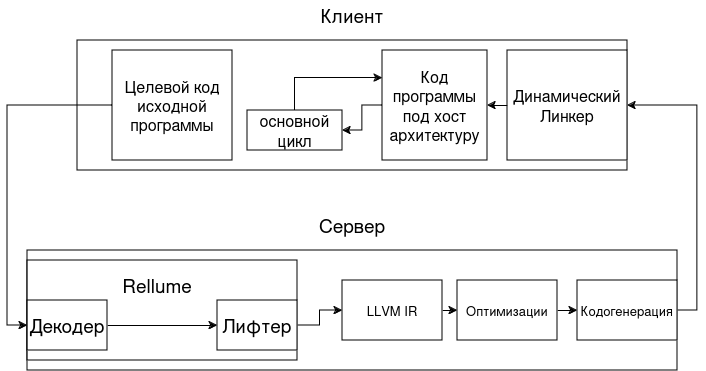
\includegraphics[width=400pt]{figures/instrew.drawio.png}
Instrew реализует клиент-сервер архитектуру:
\begin{itemize}
    \item клиент, написанный на языке C и ассемблере, и выполняющий функции:
          \begin{itemize}
              \item загрузки целевой программы в адресное пространство;
              \item эмуляции состояния процессора;
              \item отправки функций целевой программы серверу;
              \item динамической линковки ELF объектов, полученных от сервера;
              \item загрузка, разрешение символов и проведение релокаций для полученного ELF объекта;
              \item эмуляция системных вызовов;
              \item вызов функции, полученной после линковки ELF объекта;
              \item кэширование;
          \end{itemize}
    \item сервер, написанный на языке С++, выполняющий функции:
          \begin{itemize}
              \item декодирование и поднятие функции целевой программы в LLVM IR с помощью Rellume;
              \item оптимизация LLVM IR;
              \item кодогенерация;
              \item создание ELF объекта;
          \end{itemize}
\end{itemize}
% \subsection{Пример}

% \noindent Если Вам предстоит защищать учебную практику, а эти рекомендации видятся как более подходящие для защиты ВКР, то ... отмаза не засчиты\-вается, сразу учитесь делать нормально.

% % !TeX spellcheck = ru_RU
% !TEX root = vkr.tex

\section{Реализация поддержки клиента Instrew}
\begin{lstlisting}[caption={Релокация}, frame=single, breaklines, basicstyle=\footnotesize]
        uint64_t syma = (uintptr_t) sym + patch_data->addend;
        uint64_t pc = patch_data->patch_addr;
        int64_t prel_syma = syma - (int64_t) pc;

        case R_RISCV_32_PCREL:

        if (!rtld_elf_signed_range(prel_syma, 32, "R_RISCV_32_PCREL"))
           return -EINVAL;
        rtld_blend(tgt, 0xffffffffff, prel_syma);
        break;
    \end{lstlisting}

\begin{lstlisting}[caption={Заголовок}, frame=single, breaklines, basicstyle=\footnotesize]
        ASM_BLOCK(
            .text;
            .global _start;
            .type _start, %function;
        _start:
            .weak __global_pointer;
            .hidden __global_pointer;
            .option push;
            .option norelax;
            lla gp, __global_pointer;
            .option pop;
            mv a0, sp;
            .weak _DYNAMIC;
            .hidden _DYNAMIC;
            lla a1, _DYNAMIC;
            andi sp, sp, -16;
            tail __start_main;
        );
\end{lstlisting}

\begin{lstlisting}[caption={Системный вызов}, frame=single, breaklines, basicstyle=\footnotesize]
        static size_t syscall2(int n, size_t a, size_t b)
        {
            register size_t a7 __asm__("a7") = n;
            register size_t a0 __asm__("a0") = a;
            register size_t a1 __asm__("a1") = b;
            __asm_syscall("r"(a7), "0"(a0), "r"(a1))
        }
\end{lstlisting}

% % !TeX spellcheck = ru_RU
% !TEX root = vkr.tex

\section{Тестирование}
Протестировать Instrew на простых примерах не удалось, из-за сложности локализации ошибки в реализации релокаций.
% Как мы проверяем, что всё удачно получилось.
% Если работа рассчитана на несколько семестров и в текущем до эксперимента дело не дошло, опишите максимально подробно, как он будет прово\-диться и на чём
% (то, что называется \emph{дизайн эксперимента}~--- от того, что и как Вы будете проверять, очень сильно зависит, что Вы будете делать, так что это важно и делается \emph{не} после реализации).

% \subsection{Условия эксперимента}
% Железо (если актуально);
% версии ОС, компиляторов и параметры командной строки;
% почему мы выбрали именно эти тесты; входные дан\-ные, на которых проверяем наш подход, и почему мы выбрали именно их.

% \subsection{Исследовательские вопросы }
% По-английски называется \emph{research questions}, в тексте можно ссылаться на них как RQ1, RQ2, и т.~д.
% Необходимо сформулировать, чего мы хотели бы добиться работой (2 пункта будет хорошо):

% \begin{description}
%     \item[RQ1]: правда ли предложенный в работе алгоритм лучше вот таких-то остальных?
%     \item[RQ2]: насколько существенно каждая составляющая влияет на улучшения?
%           (Если в подходе можно включать/выключать какие-то составляющие.)
%     \item[RQ3]: насколько точны полученные приближения, если работа строит приближения каких-то штук?
%     \item и т.п.
% \end{description}

% Иногда в работах это называют гипотезами, которые потом проверяют.
% Далее в тексте можно ссылаться на исследовательские вопросы как \textsc{RQ}, это обще\-при\-нятое сокращение.

% \subsection{Метрики}

% Как мы сравниваем, что результаты двух подходов лучше или хуже:
% \begin{itemize}
%     \item Производительность.
%     \item Строчки кода.
%     \item Как часто алгоритм \enquote{угадывает} правильную класси\-фикацию входа.
% \end{itemize}

% \noindent Иногда метрики вырожденные (да/нет), это не очень хорошо, но если в области исследований так принято, то ладно.
% Если метрики хитрые (даже IoU или $F_1$-меру можно считать хитрыми), разберите их в обзоре, пояснив, почему выбраны именно такие метрики.

% \subsection{Результаты}

% Результаты понятно что такое.
% Тут всякие таблицы и графики, как в таблице \ref{time_cmp_obj_func}.
% Обратите внимание, как цифры выровнены по правому краю, названия по центру, а разделители $\times$ и $\pm$ друг под другом.

% Перед написанием данного раздела имеет смысл проконсультироваться с литературой по проведению экспериментов~\cite{SmirnovCheatsheet}.

% Скорее всего Ваши измерения будут удовлетворять нормальному распределению, в идеале это надо проверять с помощью критерия Кол\-могорова и т.п.
% Если критерий этого не подтверждает, то у Вас что-то сильно не так с измерениями, надо проверять кэши процессора, отключать Интернет во время измерений, подкручивать среду исполне\-ния (англ. runtime), что\-бы сборка мусора не вмешивалась и т.п.
% Если критерий удовлетворён, то необходимо либо указать мат. ожидание и доверительный/предсказы\-вающий интервал, либо мат. ожидание и среднеквадратичное отклонение, либо, если совсем лень заморачиваться, написать, что все измерения проводились с погрешностью, например, в 5\%.
% Не приводите слишком много значащих цифр (например, время работы в 239.1 секунды при среднеквадратичном отклонении в 50 секунд выглядит глупо, даже если ваш любимый бенчмарк так посчитал).

% Замечание: если у вас получится улуч\-шение производительности в пределах погреш\-ности, то это обязательно вызовет вопросы.
% Если погрешность получилась значительной (больше 10-15\% от среднего), это тоже вызовет вопросы, на которые надо ответить, либо разобравшись, что не так (первый подозреваемый~--- мультимодальное распределение), либо более глубоко статистически проанализировав результаты (например, привести гистограммы).

% В этом разделе надо также явно ответить на Research Questions или как-то их прокомментировать.

% \subsubsection{RQ1} Пояснения
% \subsubsection{RQ2} Пояснения

% \begin{table}
%     \def\arraystretch{1.1}  % Растяжение строк в таблицах
%     \setlength\tabcolsep{0.2em}
%     \centering
%     % \resizebox{\linewidth}{!}{%
%     \caption{Производительность какого-то алгоритма при различных разрешениях картинок  (меньше~--- лучше), в мс.,  CI=0.95. За пример таблички кидаем чепчики в честь Я.~Кириленко}
%     \begin{tabular}[C]{
%             S[table-format=4.4,output-decimal-marker=\times]
%             *4{S
%                         [table-figures-uncertainty=2, separate-uncertainty=true, table-align-uncertainty=true,
%                             table-figures-integer=3, table-figures-decimal=2, round-precision=2,
%                             table-number-alignment=center]
%                 }
%         }
%         \toprule
%         \multicolumn{1}{r}{Resolution} & \multicolumn{1}{r}{\textsc{TENG}} & \multicolumn{1}{r}{\textsc{LAPM}} &
%         \multicolumn{1}{r}{\textsc{VOLL4}} \\ \midrule
%         1920.1080 & 406.23 \pm 0.94 & 134.06 \pm 0.35 & 207.45 \pm 0.42  \\ \midrule
%         1024.768  & 145.0 \pm 0.47  & 39.68 \pm 0.1   &  52.79  \pm 0.1 \\ \midrule
%         464.848   & 70.57 \pm 0.2   & 19.86 \pm 0.01     & 32.75  \pm 0.04 \\ \midrule
%         640.480   & 51.10 \pm 0.2   & 14.70 \pm 0.1 & 24  \pm 0.04 \\ \midrule
%         160.120   & 2.4 \pm 0.02    & 0.67 \pm 0.01      & 0.92  \pm 0.01 \\
%         \bottomrule
%     \end{tabular}%
%     %}
%     \label{time_cmp_obj_func}
% \end{table}

% \clearpage
% \input{figures/bigtable}

% \subsection{Обсуждение результатов}

% Чуть более неформальное обсуждение, то, что сделано.
% Например, почему метод работает лучше остальных?
% Или, что делать со случаями, когда метод классифицирует вход некорректно.

% \subsection{Угрозы нарушения корректности (опциональный)}

% Если основная заслуга метода, это то, что он дает лучшие цифры, то стоит сказать, где мы могли облажаться, когда
% \begin{enumerate}
%     \item проводили численные замеры;
%     \item выбирали тестовый набор (см. \emph{confirmation bias}).
% \end{enumerate}

% Например, если мы делали замер юзабилити нашего продукта по методике System Usability Scale, но в эксперименте участвовали Ваши друзья, которые хотят Вас порадовать, честно напишите об этом.
% Честно напишите, какие меры были приняты для минимизации рисков валидности результатов эксперимента и, если это содержательно, почему их не удалось полностью исключить.

% \subsection{Воспроизводимость эксперимента}

% Это настолько важно, что заслуживает тут своего подраздела (в самой работе не надо, это должно естественно вытекать из разделов выше)~--- эксперимент должно быть можно повторить и получить примерно такие же результаты, как у Вас.
% Поэтому выложите свой код, которым мерили.
% Выложите данные, на которых мерили.
% Или напишите, где эти данные взять.
% Напишите, как конкретно запустить, в каком окружении, что надо дополнительно поставить и т.п.
% Чтобы любой второкурсник мог выполнить все пункты и получить тот же график/таблицу, что у Вас.
% Не обязательно это делать прямо в тексте, можете в README своего репозитория, но где-то надо.

% % !TeX spellcheck = ru_RU
% !TEX root = vkr.tex

\section*{Заключение}
% Список результатов, который будет либо один к одному соответствовать задачам из раздела~\ref{sec:task}, либо их уточнять (например, если было \enquote{выбрать}, то тут \enquote{выбрано то-то}).
В результате работы были выполнены следующие задачи:
\begin{itemize}
    \item проведен обзор динамических бинарных трансляторов и сравнение их с Instrew;
    \item проведен обзор архитектуры Instrew;
    \item реализована минимальная функциональность, необходимая для запуска Instrew:
          \begin{itemize}
              \item выполнены процессорно-специфичные патчи на языке ассемблера;
              \item реализована эмуляция системных вызовов;
              \item реализовано четыре архитектурно-специфичных релокаций.
          \end{itemize}
\end{itemize}

Протестировать Instrew на простых примерах не удалось, из-за сложности локализации ошибки в реализации релокаций.
Код доступен по ссылке: \href{https://github.com/mikhaylovilya/instrew/tree/host-rv64-stash}{https://github.com/mikhaylovilya/instrew/tree/host-rv64-stash}.
% \noindent Если работа на несколько семестров, отчитывайтесь только за текущий.
% Можно в свободной форме обрисовать планы продолжения работы, но не увлекайтесь~--- если работа будет продолжена, по ней будет ещё один отчёт.

% В заключении \emph{обязательна} ссылка на исходный код, если он выносится на защиту, либо явно напишите тут, что код закрыт.
% Если работа чисто теоретическая и это понятно из решённых задач, про код можно не писать.
% Обратите внимание, что ссылка на код должна быть именно в заключении, а не посреди раздела с реализацией, где её никто не найдёт.

% Старайтесь оформить программные результаты работы так, чтобы это был один репозиторий или один пуллреквест, правильно оформленный~--- комиссии тяжело будет собирать Ваши коммиты по всей истории.
% А если над проектом работало несколько человек и всё успело изрядно перемешаться, неизбежны вопросы о Вашем вкладе.

% Заключение люди реально читают (ещё до \enquote{основных} разделов работы, чтобы понять, что же получилось и стоит ли вообще работу читать), так что оно должно быть вылизано до блеска.


\setmonofont{CMU Typewriter Text}
% \bibliographystyle{ugost2008ls}
% \bibliography{vkr}

\end{document}
